\usepackage[letterpaper,landscape,margin=0.45in]{geometry}
\usepackage[T1]{fontenc}
\usepackage[utf8]{inputenc}
\usepackage{lmodern}
\usepackage{microtype}
\usepackage{xcolor}
\usepackage{tikz}
\usepackage{enumitem}
\usepackage{tabularx}
\usepackage{array}
\usepackage{multicol}
\usepackage{titlesec}
\usepackage{pagecolor}

\definecolor{aidbg}{RGB}{248,246,239}
\definecolor{aidtext}{RGB}{28,28,28}
\definecolor{unionaccent}{RGB}{58,96,145}
\definecolor{unionfill}{RGB}{228,236,247}
\definecolor{confaccent}{RGB}{131,44,39}
\definecolor{conffill}{RGB}{228,220,214}
\definecolor{panelrule}{RGB}{120,120,120}

\pagecolor{aidbg}
\color{aidtext}
\setlength{\parindent}{0pt}
\setlength{\parskip}{0.35em}
\setlist[itemize]{leftmargin=1.2em,itemsep=0.15em,topsep=0.15em}
\pagestyle{empty}

\titleformat{\section}
  {\Large\bfseries}
  {}
  {0pt}
  {}

\newcommand{\aidtitle}[2]{%
  {\centering
  {\fontsize{22}{24}\selectfont\bfseries #1\par}
  \vspace{0.2em}
  {\large\itshape Shenandoah: Valley of Fire\par}
  \vspace{0.5em}
  \color{#2}\rule{\textwidth}{1.2pt}\par
  }\vspace{0.75em}
}

\newcommand{\sequencepanel}{%
  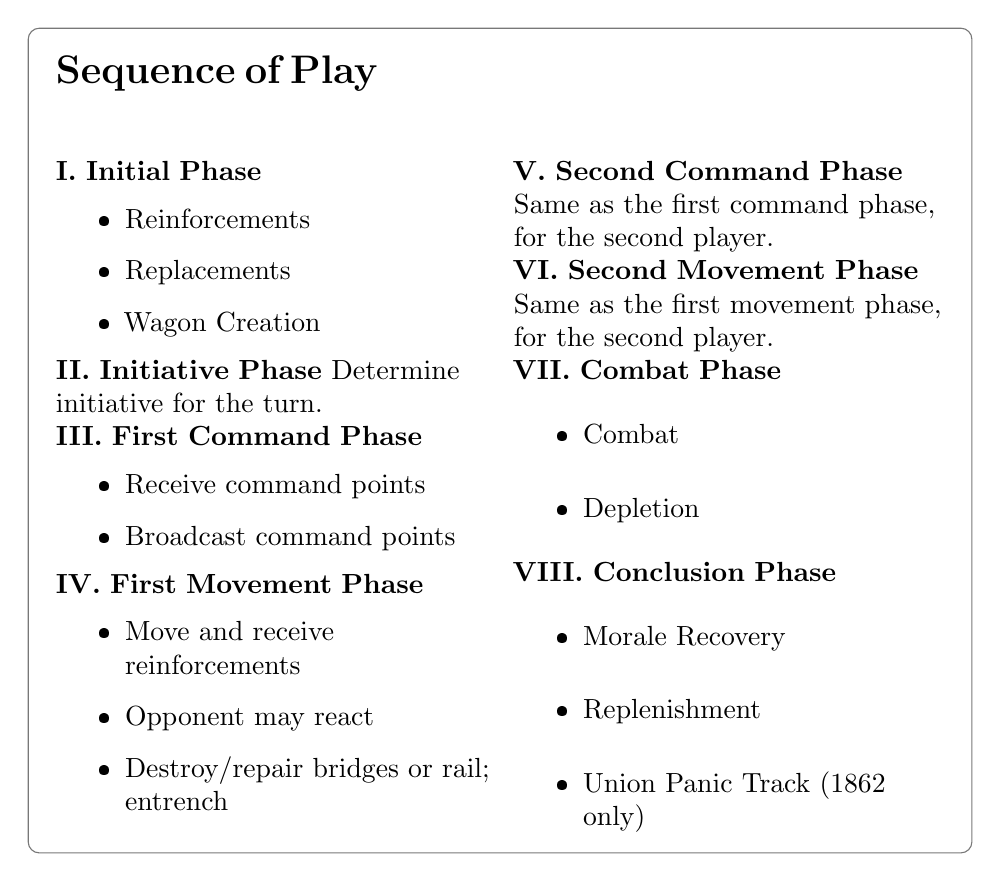
\begin{tikzpicture}
    \node[draw=panelrule,rounded corners=4pt,fill=white,inner sep=10pt,text width=\textwidth-24pt] (panel) {%
      {\Large\bfseries Sequence of Play}\par\vspace{0.4em}
      \begin{multicols}{2}
      \textbf{I. Initial Phase}
      \begin{itemize}
      \item Reinforcements
      \item Replacements
      \item Wagon Creation
      \end{itemize}
      \textbf{II. Initiative Phase}
      Determine initiative for the turn.

      \textbf{III. First Command Phase}
      \begin{itemize}
      \item Receive command points
      \item Broadcast command points
      \end{itemize}

      \textbf{IV. First Movement Phase}
      \begin{itemize}
      \item Move and receive reinforcements
      \item Opponent may react
      \item Destroy/repair bridges or rail; entrench
      \end{itemize}

      \columnbreak

      \textbf{V. Second Command Phase}
      Same as the first command phase, for the second player.

      \textbf{VI. Second Movement Phase}
      Same as the first movement phase, for the second player.

      \textbf{VII. Combat Phase}
      \begin{itemize}
      \item Combat
      \item Depletion
      \end{itemize}

      \textbf{VIII. Conclusion Phase}
      \begin{itemize}
      \item Morale Recovery
      \item Replenishment
      \item Union Panic Track (1862 only)
      \end{itemize}
      \end{multicols}
    };
  \end{tikzpicture}%
}

\newcommand{\holdingbox}[3]{%
  \begin{tikzpicture}
    \node[
      draw=#2,
      line width=1.2pt,
      rounded corners=4pt,
      fill=#3,
      minimum width=2.1in,
      minimum height=1.35in,
      inner sep=0pt
    ] {\fontsize{18}{20}\selectfont\bfseries #1};
  \end{tikzpicture}%
}

\newcommand{\holdingnote}{%
  \vspace{0.5em}
  {\small Units placed in a holding box are considered to occupy the same hex as the named leader.}
}
